\label{B1DATASECTION}
The HERMES collaboration  made the first measurement~\cite{Airapetian:2005cb} of
the inclusive tensor structure function $b_1$ in 2005.
The experiment explored the kinematic range of $0.001<x<0.45$ for  $0.5<Q^2<5$ GeV$^2$.  
An atomic beam source was used to generate a deuterium gas target with high tensor polarization.  
The HERA storage ring provided 27.6 GeV positrons incident on the internal gas target.

The tensor asymmetry A$_{zz}$  was found to be non-zero by about two sigma  for $x < 0.1$, and 
the tensor structure function  $b_1$ displayed a steep rise as $x\to 0$.
The CK integral was evaluated and found to be 
\begin{eqnarray}
\int_{0.0002}^{0.85} b_1(x) dx = 0.0105 \pm 0.0034 \pm 0.0035
\end{eqnarray}
which result possibly indicates a breaking of the Close-Kumano sum rule, and consequently a 
tensor-polarized quark sea.
%
%
\begin{figure}[h]
\begin{center}
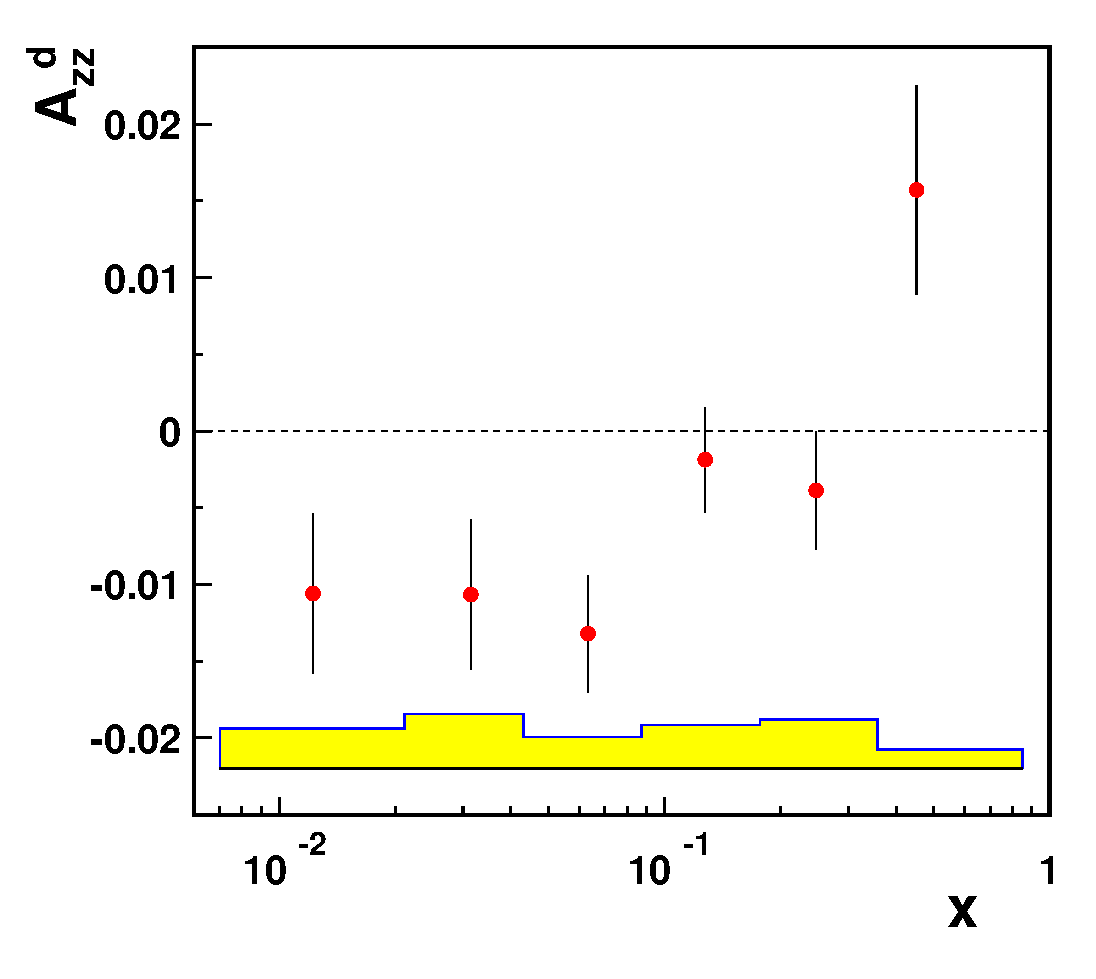
\includegraphics[angle=0,width=4.in]{figs/azzfinal.eps}
\caption{\label{HERMES_AZZ} HERMES measurement of the inclusive tensor asymmetry A$_{zz}$ of the deuteron.  
The error band displays the total systematic uncertainty.
{\it Reproduced from~\cite{Riedl:2005jq}.}}
\end{center}\end{figure}

As often the case with pioneer measurement, the precision of the results leaves
room for ambiguities on the type of phenomena which are responsible for a non-zero 
value of $b_1$.
One worry is that HERMES $Q^2$ values are low at small $x$ (see Fig.~\ref{HERMES_KIN}) 
where quark structure functions may not be the correct language. In addition the $Q^2$ 
coverage in each $x$-bin is quite wide and could mask any $Q^2$-dependence.
Indeed, several theoretical models, as for example displayed in Fig.~\ref{xb1_pred},
show a significant $Q^2$-dependence for $x \le 0.1$.


\begin{figure}
\begin{center}
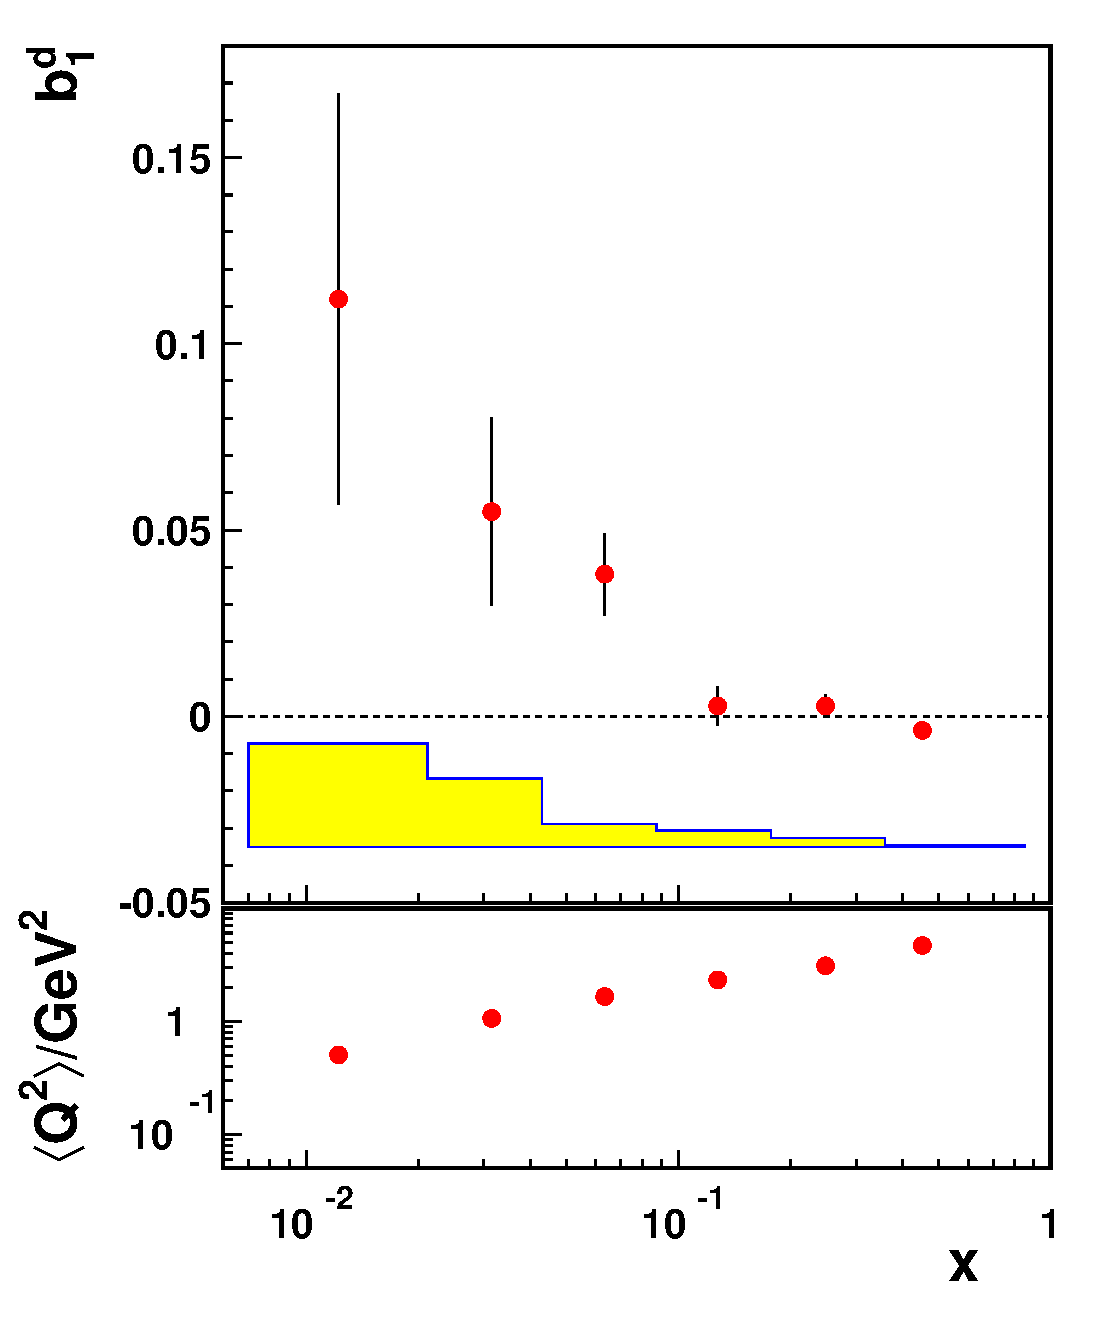
\includegraphics[angle=0,width=4.1in]{figs/b1final.eps}
\caption{\label{HERMES_B1D} HERMES measurement of the inclusive tensor structure function b$_1^d$ and the average $Q^2$ for each x-bin.  The error band displays the total systematic uncertainty.
{\it Reproduced from~\cite{Riedl:2005jq}.}}
\end{center}\end{figure}


\begin{figure}
\begin{center}
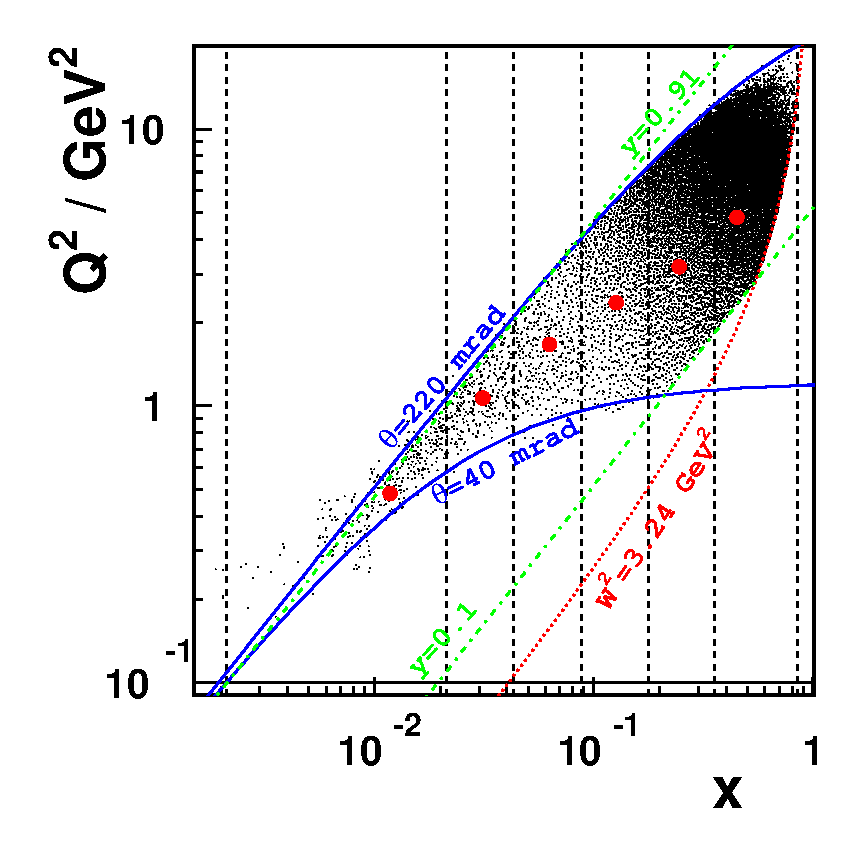
\includegraphics[angle=0,width=4.in]{figs/kineplane.eps}
\caption{\label{HERMES_KIN} Kinematic coverage of the HERMES measurement.  The dashed vertical lines indicate the borders 
of the bins in x, the big dots their centers of gravity. The solid curves 
indicate the 
vertical acceptance of the spectrometer, defined by its apperture. 
In addition, the 
kinematic cuts imposed on the variables Q$^2$, y 
and W$^2$ are shown. The W$^2$
cut suppresses the nuclear resonance region. 
{\it Reproduced from~\cite{Riedl:2005jq}.}}
\end{center}\end{figure}


%\begin{figure}\begin{center}
%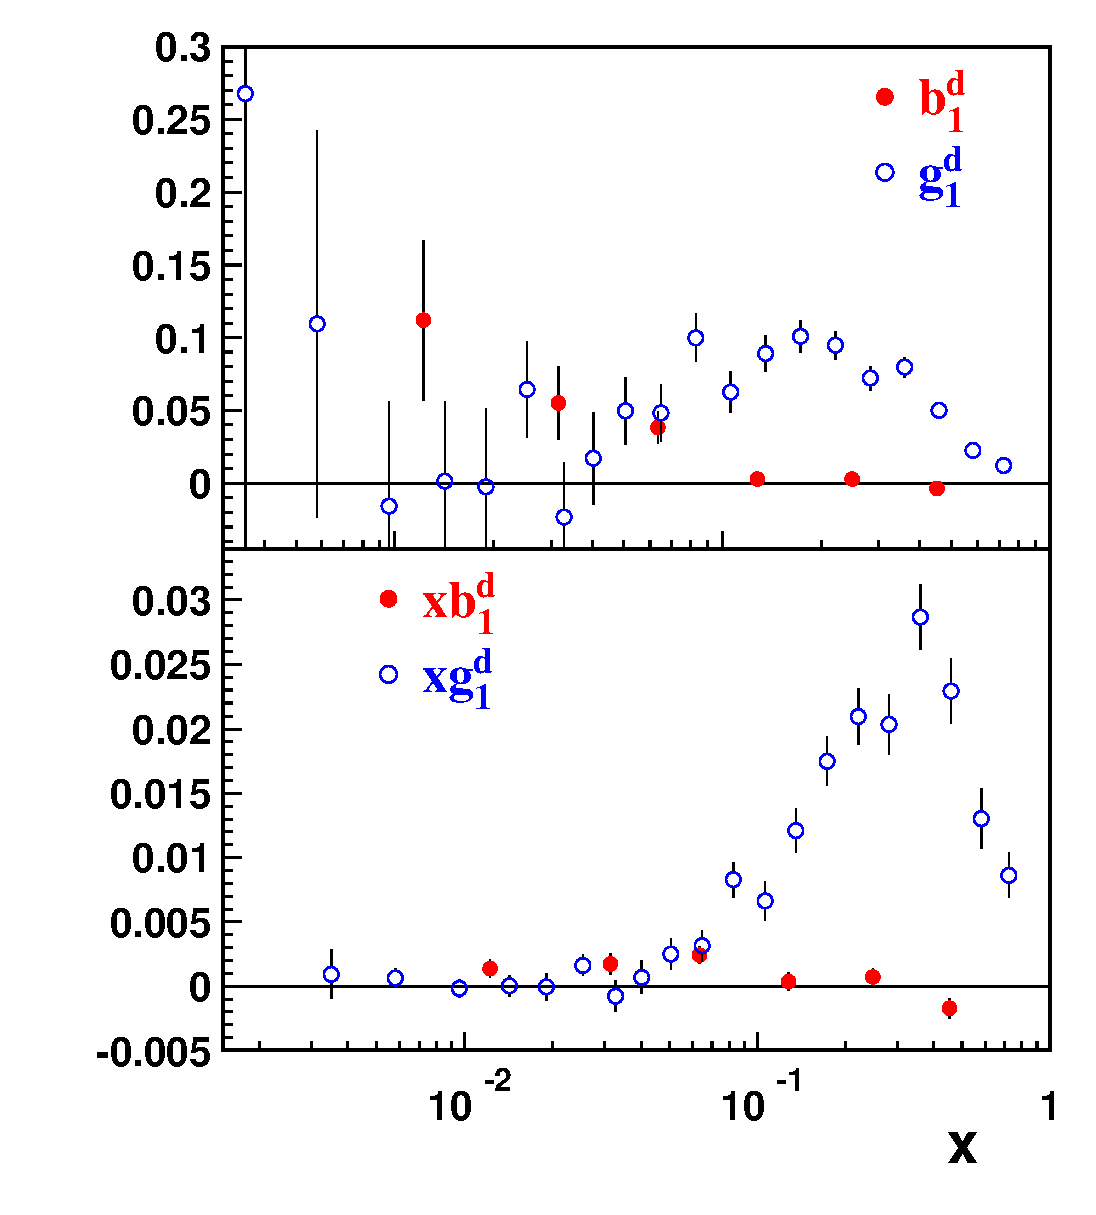
\includegraphics[angle=0,width=3.1in]{figs/b1g1.eps}
%\caption{\label{}\footnotesize
%{\it Reproduced from~\cite{Riedl:2005jq}.}}
%\end{center}\end{figure}

%\begin{figure}\begin{center}
%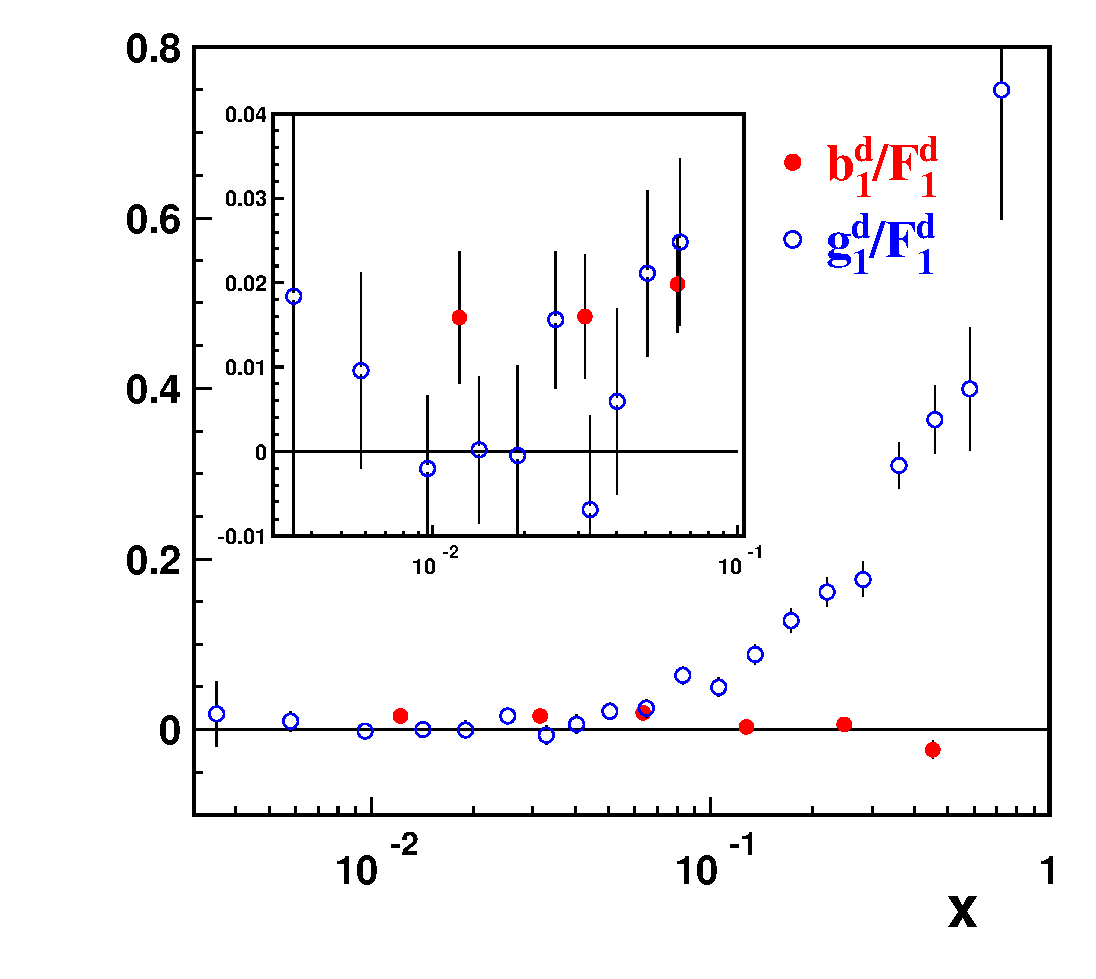
\includegraphics[angle=0,width=3.1in]{figs/b1g1overf1.eps}
%caption{\label{}\footnotesize
%{\it Reproduced from~\cite{Riedl:2005jq}.}}
%\end{center}\end{figure}

%\begin{figure}\begin{center}
%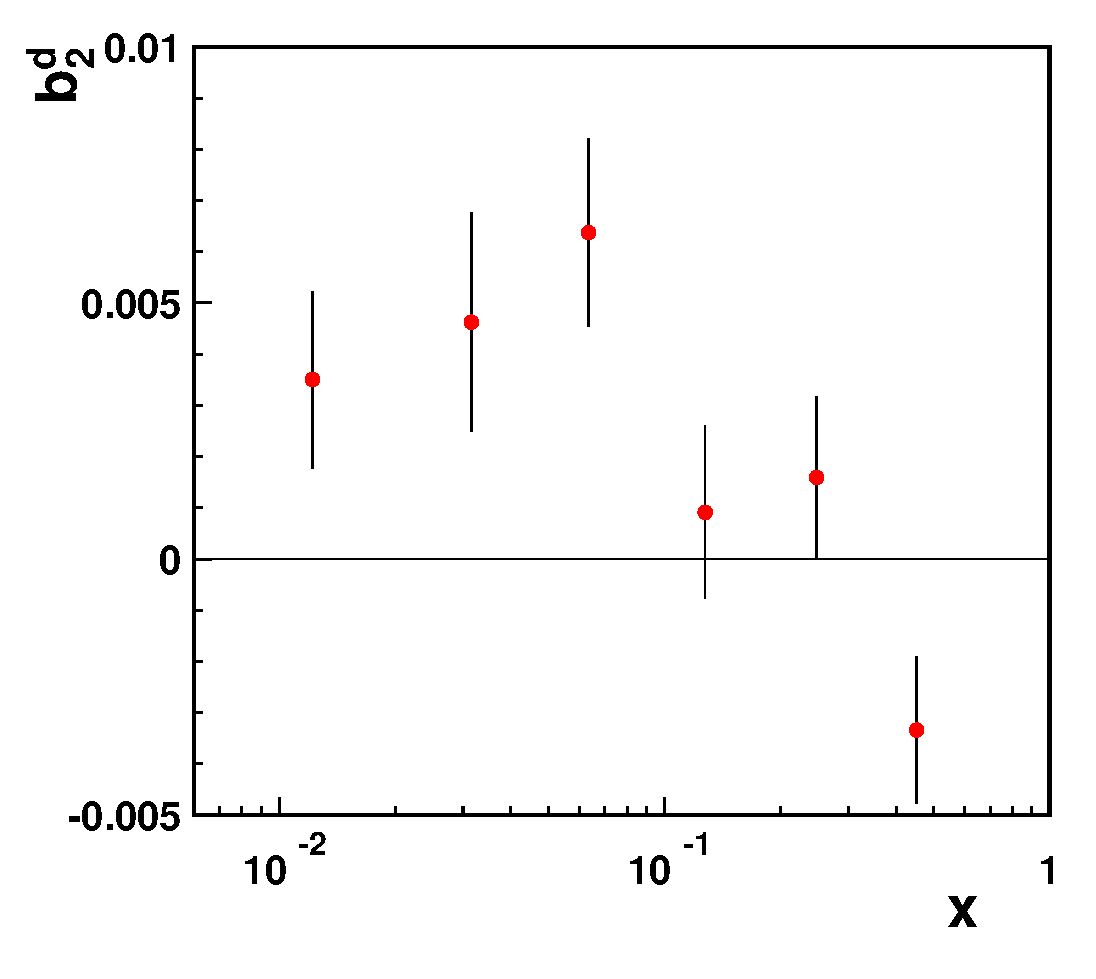
\includegraphics[angle=0,width=3.1in]{figs/b2theo.eps}
%\caption{\label{}\footnotesize
%{\it Reproduced from~\cite{Riedl:2005jq}.}}
%\end{center}\end{figure}

